\section{Simulation results}

The PMSM model introduced in chapter \ref{PMSM model} is used in the simulations. The flux linkages are defined as \eqref{Eq:flux-linkages} and the stator voltages as \eqref{Eq:voltage}. Iron losses are not modelled. Simulations are performed by time-stepping. Speed calculations are based on the equation of motion \eqref{PMSM_dynamics}.

Evaluation was done by capturing data in three different cases. In the first case, the data was captured using only a PI speed controller. In the second and third cases, the data was captured by having the PI-controller coupled with ILC and Q-learning based compensators, respectively. Everything else was kept unchanged. Hence, the data captured using only the conventional PI-controller, works as a basis for the performance evaluation.

%\begin{equation}
%    TR = \frac{T_{max} - T_{min}}{T_{avg}}
%    \label{eq:ripple}
%\end{equation}
The speed and torque ripples can be measured, which allows fair evaluation of compensation effectiveness. The evaluation is done using a speed ripple factor (SRF) and a torque ripple factor (TRF). These are defined as \cite{ILC:2005}
\begin{align}
    \text{SRF} &= \frac{\omega_{max} - \omega_{min}}{\omega_N} \cdot 100\% & \text{TRF} &= \frac{T_{max} - T_{min}}{T_N} \cdot 100\%
    \label{eq:ripple-factor}
\end{align} 
where peak-to-peak values are obtained from a single period. In addition to the SRF and the TRF, the amplitudes of $1$st, $2$nd, $6$th, $12$th harmonics are compared as these are pertinent to assessment. Simulations are performed with the motor described in Table \ref{Tbl:MS4887}.

%Performance can be assessed by calculating speed and torque ripple ratios, as was done in \cite{ILC:2012}. The ratios can be calculated by dividing SR or TR measures of two cases. In the first case, the compensator is enabled and in the second case, plain PI-controller is used.
%\begin{align}
    %SRR &= \frac{SR_{compensated}}{SR_{uncompensated}} & TRR &= \frac{TR_{compensated}}{TR_{uncompensated}}
%\label{eq:ripple-ratio}
%\end{align}
%This measure allows fair comparison between the results. The performance is also evaluated by inspecting the magnitudes of significant harmonics.



%Torque pulsations were summed to simulator torque calculation, thus causing the total torque to fluctuate. The compensators were used to dampen the occurring pulsations, which allowed the evaluation of the performance. 


%Even if single harmonic may not resemble exactly sine wave, their coaction can be approximated by a Fourier series expansion \cite{Observer:2013}.

\begin{table}[ht]
\caption{MS4887 motor nameplate values}
\centering
\begin{tabular}[t]{lccc}
\hline
Description & Symbol & Value  & Unit\\
\hline
Nominal current (rms) & $I_N$ & 18.1  & A\\
Nominal voltage (rms, line-line)  & $U_N$  & 195.1 & V\\
Nominal frequency & $f_N$      & 133.3 & Hz\\
Nominal speed     & $\omega_N$ & 2000  & rpm\\
Nominal power     & $P_N$      & 6     & kW\\
Nominal torque    & $T_N$      & 28.6  & Nm\\
Number of poles   & $N_p$      & 8     & \\
\hline
\label{Tbl:MS4887}
\end{tabular}
\end{table}%

\subsection{Torque pulsation model}
% cogging \cite{CTR_HW:2002, CTR_HW:2004, CTR:2010, CTR_HW_skew:2013, CTR_SW:2017, CTR_HW:2017}
%It was found that all the relevant torque ripple sources are periodic. This allows the pulsations to be modeled by using Fourier series, which makes the generation of the desired harmonics simple. Only magnitude and frequency information of the pulsations is needed. Since the pulsation magnitudes have dependency on the motor, the magnitudes must be either calculated, measured or estimated. 

%The general representation of Fourier series is given by
%\begin{equation}
%    T(t) = T_0 + \sum_{n=1}^{\infty} T_n \cos(n \omega_1 t + \phi_n)
%    \label{pulsation_model1}
%\end{equation}
%The representation can be made more practical for torque pulsation generation purposes. The frequency can be expressed by using rotor angle, since the angular speed can be derived from the angle and there is a relationship between the angular speed and frequency ($\omega = 2 \pi f$). This allows the formula to be written as

In order to be able to evaluate compensation performance in the simulator, disturbances must be generated. Since torque pulsation needs to be only periodic, these can be modelled by using Fourier series
\begin{equation}
    T_m(\theta_e) = \sum_{n=1}^{\infty} T_n \cos(n \theta_e + \phi_n)
    \label{pulsation_model2}
\end{equation}  % \cite{CTR_SW:1998}
where $T_n$ is the magnitude of the $n$th harmonic and $\phi_n$ is the phase shift. The phase shift can be assumed to be zero for simplicity, as $\phi_n$ has no effect to compensation results. In order to make the model more practical, only harmonics incorporating significant amount of energy, i.e., $\{ 1, 2, 6, 12\}$ are used for modelling the pulsations. This scheme requires only a few amplitudes to be specified in order to model pulsations. With more complex models, it was found that lack of details, such as stator slot number, can prevent modelling entirely.

%Imitating the torque pulsations of different motors by using the previous model is easy. Only the order of harmonics must be known accurately. The magnitudes can be estimated whereas the rotor position information should be always known, since the compensators cannot work without it. The little amount of required information is very beneficial as it allows to model a lot of different motors with little effort. With more complex models, it was found that the lack of motor details, such as number of stator slots, may prevent modelling. 

%An example of generated pulsations is shown in Fig. \ref{fig:ilc_concept}.
%The temperature has effect on magnitude of cogging torque \cite{CTR_SW_ff:2011}.

%Speed controller gains were set to $K_p = 10$ and $K_i = 1.5$. The same PI gains were used in all tests.

%It was found that Angle-based ILC can be kept enabled during transients without problems, although doing so may not be advisable *citations*.

%\subsection{Operating conditions}

% measured 80% load
The harmonic magnitude $T_n$ must be measured, computed or estimated by utilizing available information. For realistic simulations, the magnitudes were measured at high load from one of the motors used in the experiments. Harmonics $T_1$, $T_2$, $T_6$ and $T_{12}$ were obtained using a torque transducer and then calculating FFT. Harmonic magnitudes are listed in Table \ref{Harmonics}.
\begin{table}[tb]
\caption{Modelled harmonics with respect to nominal torque}
\centering
%\scalebox{0.9}{%
\begin{tabular}[t]{lcccccc}
\hline
Harmonic order   & 1st & 2nd & 6th & 12th \\
\hline
Magnitude (\%)   & \num{1.37} & \num{0.25} & \num{0.45} & \num{0.09} \\
\hline
\label{Harmonics}
\end{tabular}%}
\end{table}%
It can be observed that the $12$th harmonic already incorporates very little energy. Therefore, exclusion of less significant harmonics should not introduce much error. A similar conclusion was made in \cite{CTR_SW:1998}.

All simulations were made at $60$ rpm speed, because pulsations degrade motor performance the most at low speeds. This can be reasoned by inspecting \eqref{Eq:transfer_function} and its frequency response. With higher frequencies, the speed oscillations diminish spontaneously, thus making low speed compensation more critical. In order to make simulations more realistic, white noise was added to the speed signal. This was done similarly to chapter \ref{hyperparameters}, though more restrained $10\%$ amplitude was used for generating the noise. Due to added noise, the compensator speed input can vary between $54-66$ rpm when the measured speed stays constant $60$ rpm.
%The pulsations were studied only in no-load operating conditions to limit the number of simulations. Greater amount of space is reserved for experimental results that may be more interesting.
%The performance has been also studied experimentally and these results may be more interesting, thereby more space is reserved for these results.
%The simulator was run for $500$ seconds before capturing the data

\subsection{Results with fine tuned compensators} \label{Results with fine tuned compensators}

In the first simulation, both compensators were fine tuned. Many test simulations were performed in order to find good parameter values before evaluation. It was found that ILC performs well with parameter values of $\Phi = 9$, $\Gamma = 3$ and $\alpha = 0.05$. ILC memories were set to store $750$ values. According to simulation results in Figs. \ref{fig:lambda}, \ref{fig:alpha}, \ref{fig:gamma} and \ref{fig:glie}, the Q-learning based compensator performs well with parameter values given in Table  \ref{Tbl:Q-params}. In addition to the table values, the torque pulsation maximum was set to $T_{max}=0.014$. Seven actions and 100 states were used in order to keep memory consumption roughly equivalent to ILC, thus allowing more fair comparison. Better compensation performance could be achieved with both compensators, if more memory was reserved for storing values.

\begin{table}[b]
\caption{Parameter values used with Q-learning}
\centering
%\scalebox{0.9}
\end{table}%

The ripple factors were calculated from simulation data. When using only a conventional PI controller, the measures are SRF = $0.21$\% and TRF = $11.8$\%. With ILC enabled, the corresponding measures are SRF = $0.04$\% and TRF = $11.6$\%. With Q-learning, SRF = $0.05$ \% and TRF = $10.8$\%. Ripple factors show that pulsations do get significantly reduced when compensators are enabled. SRF reduction is much greater than TRF. Reason for this can be observed from Fig. \ref{sim:results-time}, which shows that the torque signal is much noisier than the speed signal due to system dynamics \eqref{Eq:transfer_function}. The speed signal behaves similarly to a low-pass filtered signal, which makes the SRF measure more reliable than TRF. Peak values used for calculating the ripple factor are more consistent with the speed signal than they are with torque. The overall ripple is clearly getting reduced even with the torque signal, but singular spikes in the data can still keep the TRF measure high. It can be concluded that the SRF measure should be favoured over the TRF, since the SRF measure is more consistent.

Harmonic magnitudes in Fig. \ref{sim:well-tuned} allow to make the same conclusion as can be made from the SRF and TRF measures. Compensators reduce pulsations, since harmonics are much smaller when compensators are enabled. Speed harmonics are reduced more than torque harmonics similarly to SRF and TRF measures. It can be observed that Q-learning based method is not able to compensate the first speed harmonic as well as ILC. Since the first harmonic has the greatest magnitude, it has the greatest effect on the ripple. This explains why ILC manages to compensate pulsations more according to the SRF measure. In case of torque harmonics, the Q-learning based method appears to be able to compensate torque harmonics better in overall than ILC, hence leading to smaller TRF.
\begin{figure}[htb] 
    \centering
    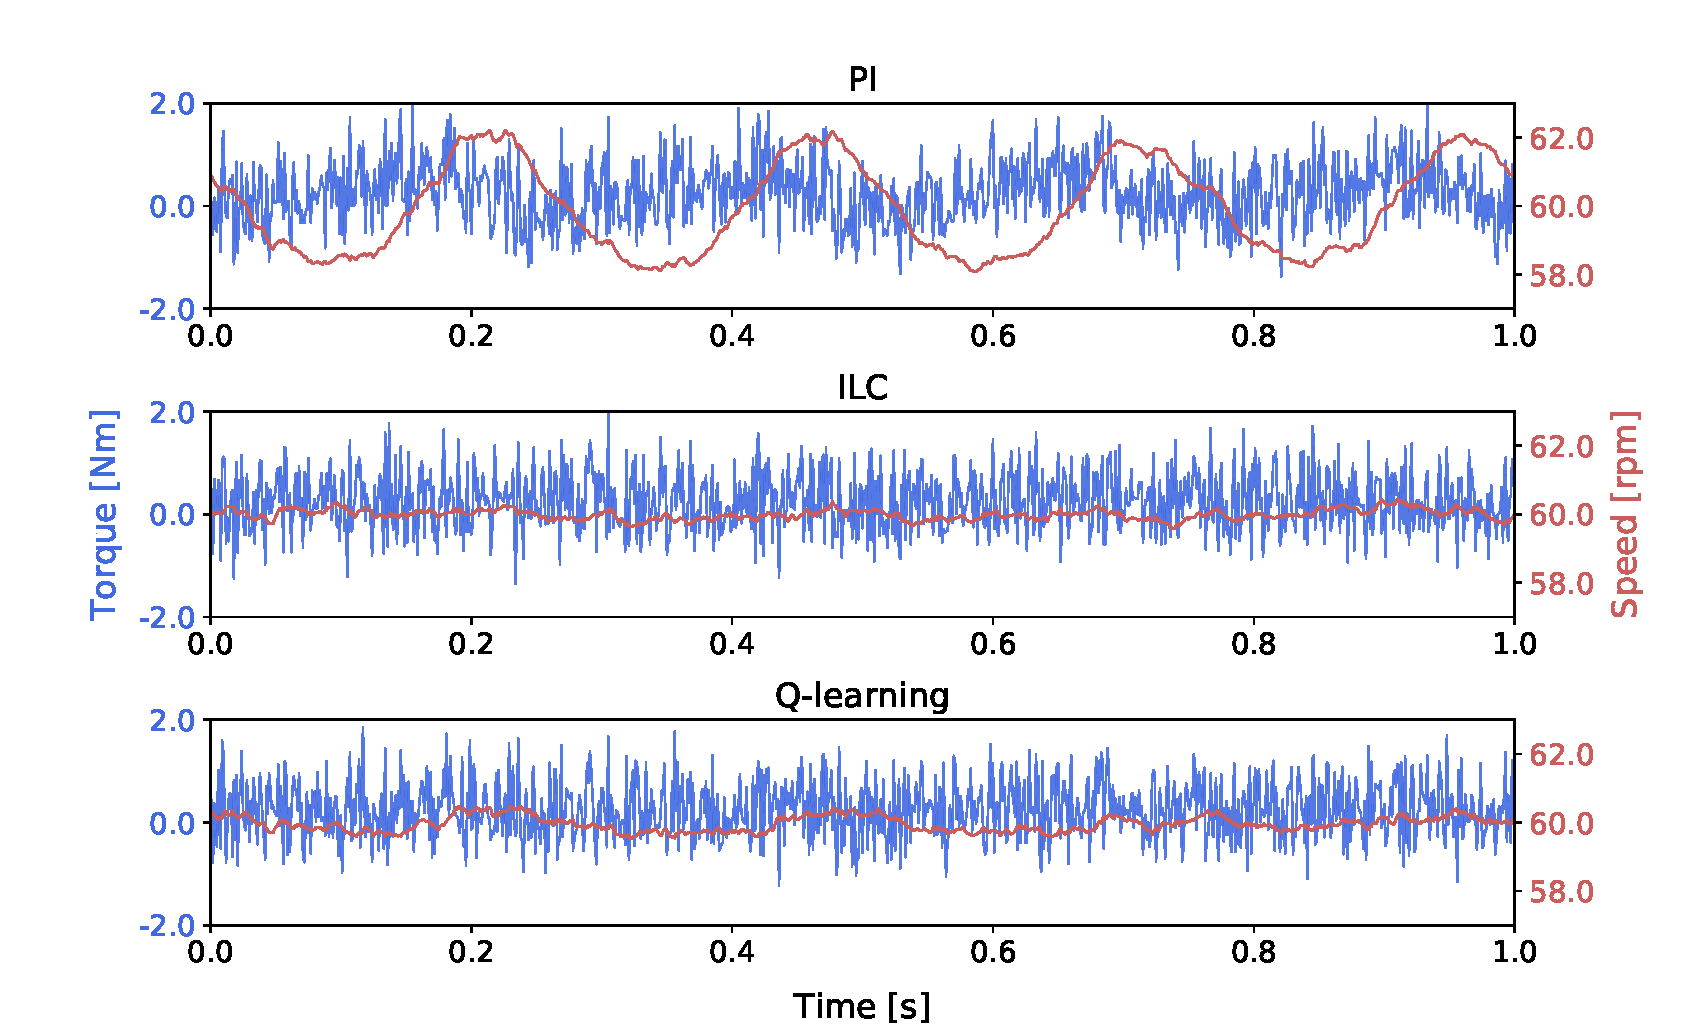
\includegraphics[width=1.0\textwidth]{images/simulation-results-time.pdf}
    \caption{Simulated torque and speed pulsations with PI, ILC and Q-learning compensation schemes}
    \label{sim:results-time}
\end{figure}


%With specified parameters, ILC data storing scheme consumes roughly $5.86$ KB memory whereas Q-value tables use $5.47$ KB with $32$ bit floating point numbers.
\begin{figure}[htb]
\centering
\begin{subfigure}{0.5\textwidth}
  \centering
  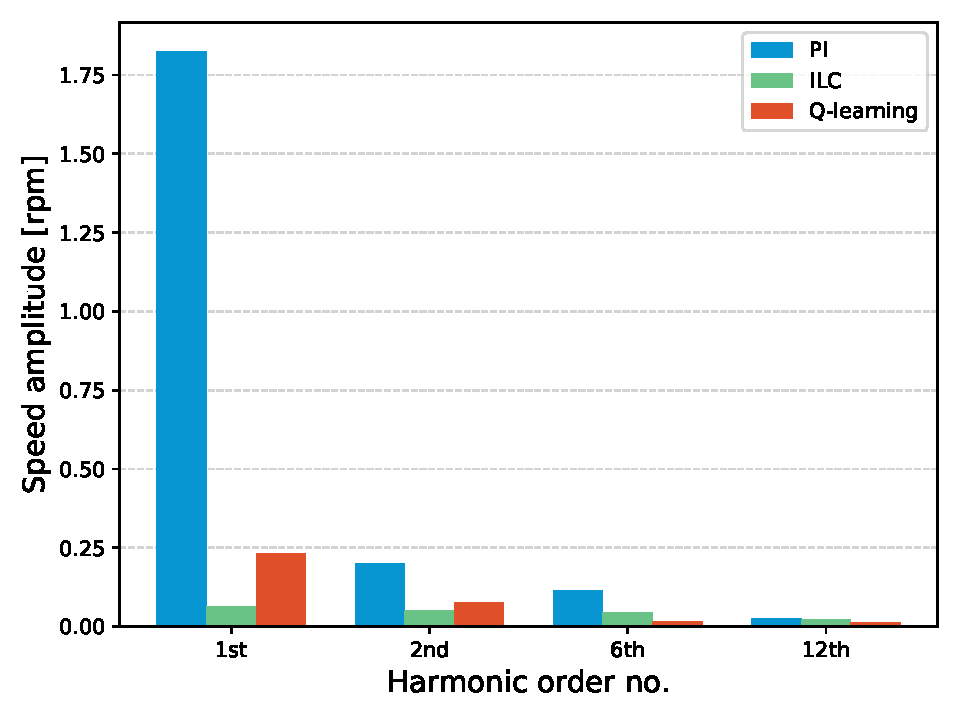
\includegraphics[width=\textwidth]{images/simulations_ms4887_tuned_speed_pi_ilc_qlr.pdf}
  \caption{Speed harmonics}
\end{subfigure}%
\begin{subfigure}{.5\textwidth}
  \centering
  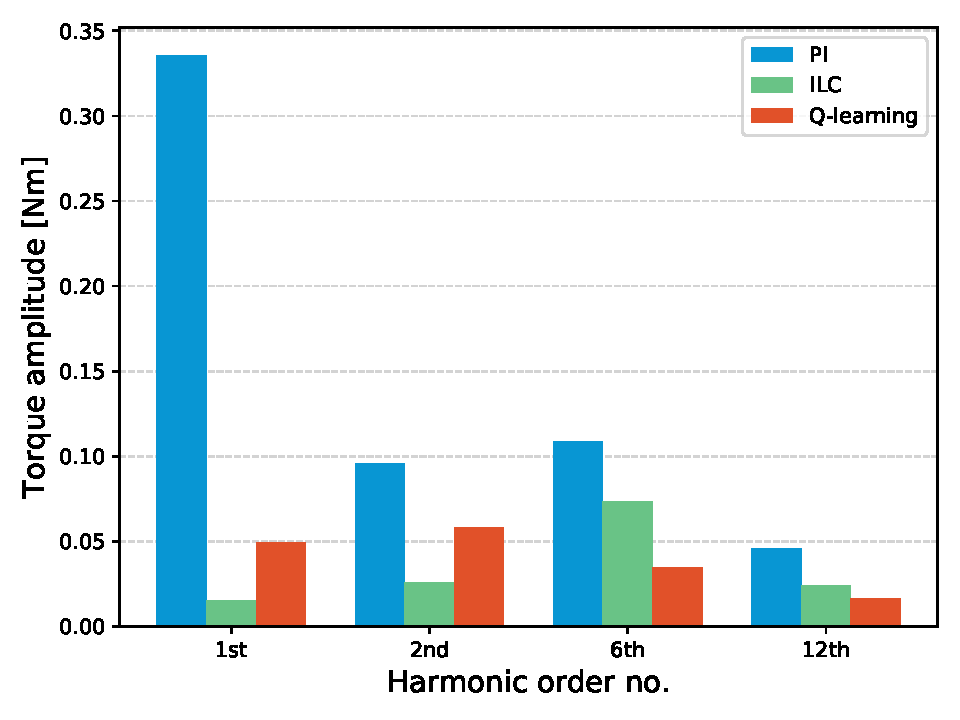
\includegraphics[width=\textwidth]{images/simulations_ms4887_tuned_torque_pi_ilc_qlr.pdf}
  \caption{Torque harmonics}
\end{subfigure}
\caption{Speed and torque harmonics of fine tuned compensators}
\label{sim:well-tuned}
\end{figure}
The simulation result supports previous studies. In \cite{ILC:2005}, ILC was tested experimentally. The SRF measure without compensation was $0.65\%$ and with compensation $0.15\%$. A ripple reduction ratio can be calculated from these percentages, which allows to compare the performance with the simulation result. By calculating ratios, $0.15\% / 0.65\% \approx 0.23$ and $0.043\% / 0.206\% \approx 0.21$ it can be observed that compensation performance is quite similar.

%PI-SRF = 0.206 \%
%ILC-SRF = 0.043 \%
%QLR-SRF = 0.048 \%
%PI-TRF = 11.8
%ILC-TRF = 11.6
%QLR-TRF = 10.8

%the $1$st, $2$nd and $6$th harmonics significantly. Q-learning based solution did not seem to reduce the $12$th harmonic, but this is not surprising. The harmonic magnitude is already small and it has the highest frequency of considered harmonics, thus its compensation is most difficult and produces least reward. Therefore, the Q-learning based compensator may favor compensation of lower harmonics, which is fine outcome, since the harmonics having highest magnitude and lowest frequency are often the most problematic ones. If some harmonics were particularly important to compensate for, then this could be specified in the reward function. Q-learning based compensator manages to reduce $2$nd and $6$th harmonics even more than ILC, which already demonstrates the potential of the method. ILC reduced first harmonic more.



% \subsection{Speed ramp without load (?)}

% \subsection{Speed ramp with load (?)}
\subsection{Results with nonideal parameters}
Another simulation was made with more realistic parameter values. It is unfeasible to assume that maximum torque amplitude is known beforehand, therefore nonideal value of $T_{max}=0.01$ was intentionally used. The ILC gains in the previous simulation were higher than it is usually possible to use with a real motor. Hence, lower gains of $\Phi = 4.75$ and $\lambda = 1.0$ were selected for the simulation. Additionally, a higher forgetting factor $\alpha = 0.15$ value was used with ILC. Other parameters and operating conditions were kept the same as in the previous simulation.

Figure \ref{sim:torque-ripple} shows that disturbances are getting reduced when compensators are used. The $1$st and $2$nd harmonics can be clearly seen to get smaller when comparing Figs. \ref{sim:a} and \ref{sim:b} to \ref{sim:c}. Also $6$th harmonic is getting reduced when Q-learning based compensator is used. The $12$th harmonic reduction is not clear due to noisy appearance of the torque signal and low energy of the $12$th harmonic. Since harmonics are getting smaller, it can be concluded that compensators are able to reduce torque ripple with nonideal parameter values. The compensation performance is worse than with fine compensators in Fig. \ref{sim:well-tuned}, but this is fully expected, as some q-axis current reference injections are simply too small.

The green signal in Figs. \ref{sim:a} and \ref{sim:b} illustrates the torque that gets produced when compensators correct the q-axis current reference, $i_q^*$. The compensation torque allows to observe that both compensators successfully identify periodic pulsations, because produced torque harmonics overlap with harmonic orders of the disturbances. Besides $1$st, $2$nd, $6$th and $12$th harmonics, the Q-learning based method can be seen to generate also other minor harmonics. The rise of these minor harmonics can be explained with the rough compensation pattern, which is visualized in Fig. \ref{fig:learned_pattern_torque}. The compensator cannot generate ideal waveform needed for compensation due to quantization of the actions. ILC can inject any real value, which explains why ILC generates less these superfluous compensation harmonics. The almost nonexistent superfluous harmonics in case of ILC are caused by noise, which prevents precise disturbance identification. Anyhow, these superfluous harmonics are harmless in both cases, since their amplitude is tiny compared to prominent harmonics.

\begin{figure}[hb]
\begin{subfigure}{.5\linewidth}
\centering
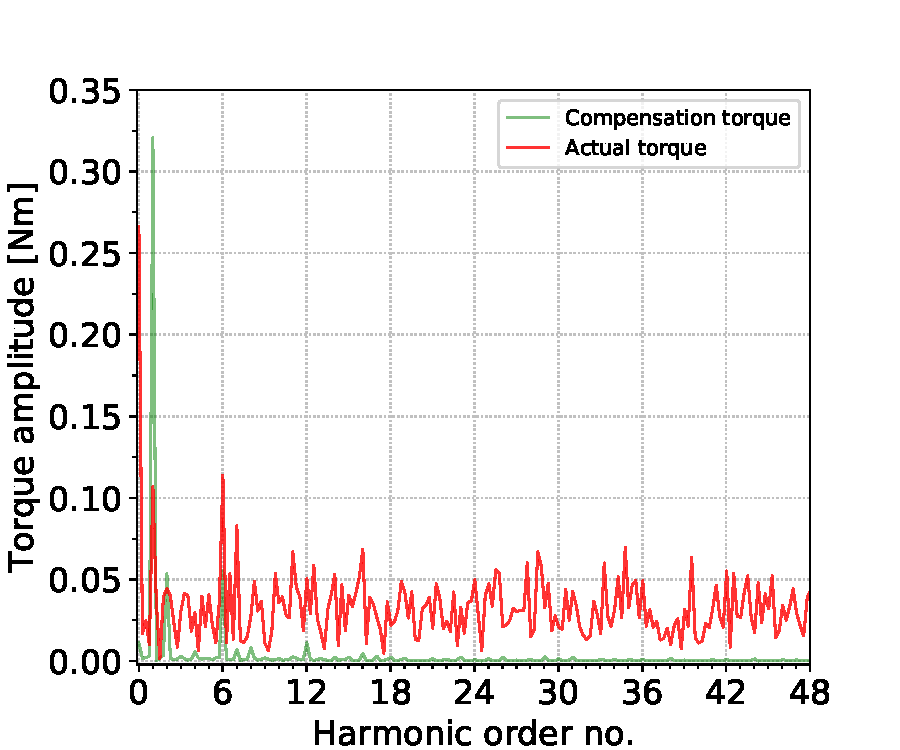
\includegraphics[width=\textwidth]{images/b-sim-ilc-enabled.pdf}
\caption{ILC}
\label{sim:a}
\end{subfigure}%
\begin{subfigure}{.5\linewidth}
\centering
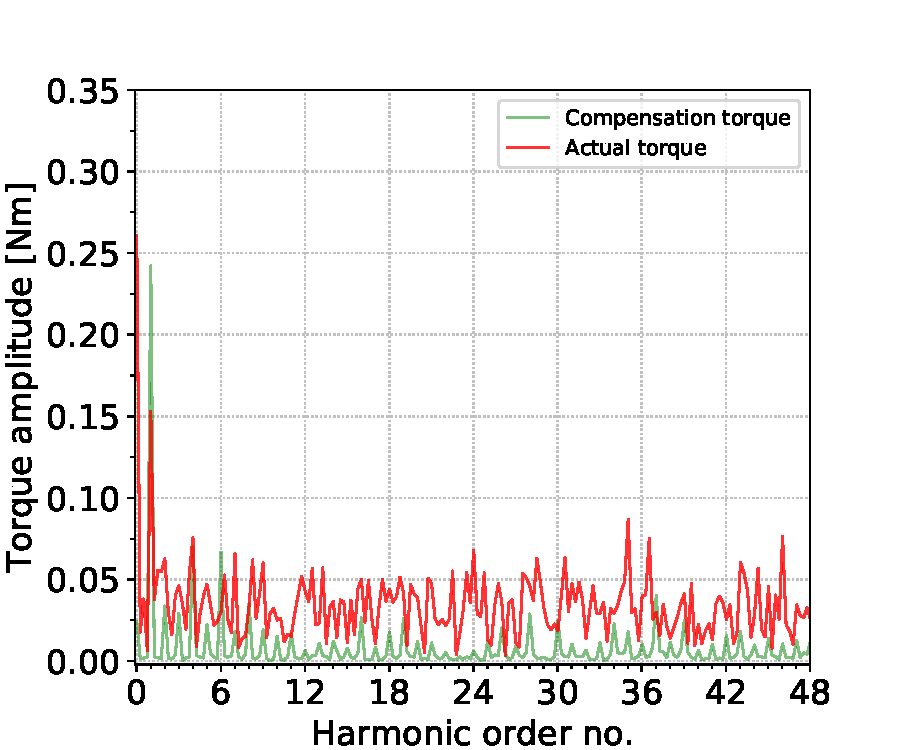
\includegraphics[width=\textwidth]{images/b-sim-qlr-enabled.pdf}
\caption{Q-learning}
\label{sim:b}
\end{subfigure}\\[1ex]
\begin{subfigure}{\linewidth}
\centering
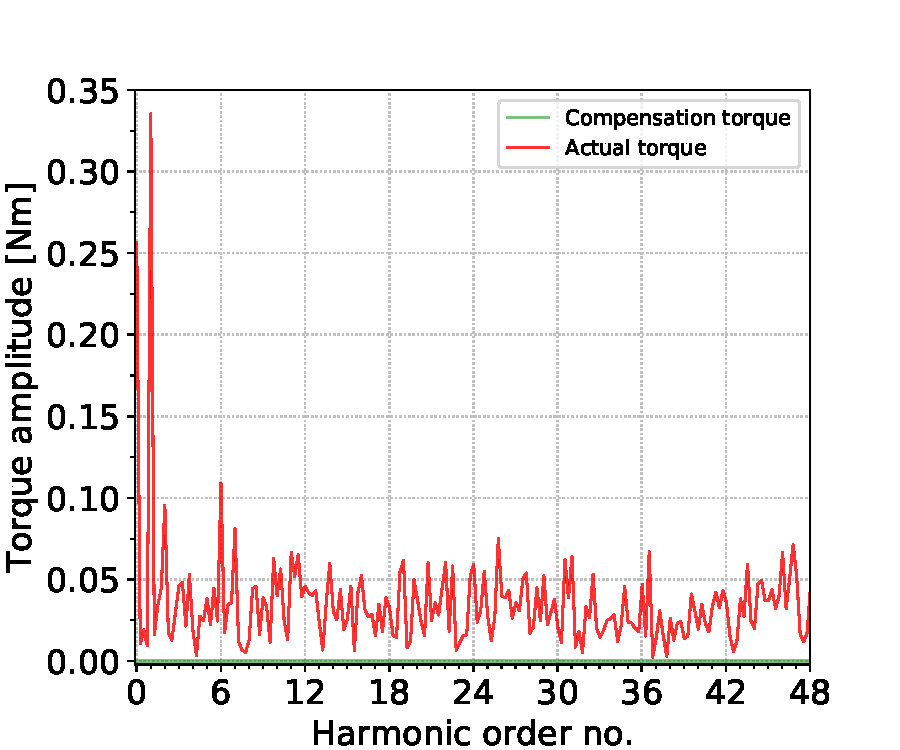
\includegraphics[width=.5\textwidth]{images/a-sim-ilc-disabled.pdf}
\caption{PI control}
\label{sim:c}
\end{subfigure}
\caption{Simulated torque harmonics when (a) ILC compensator is used (b) Q-learning based compensator is used and (c) conventional PI speed control is used}
\label{sim:torque-ripple}
\end{figure}


%ILC-SRF = 0.00085
%QLR-TRF = 0.00119
%ILC-TRF = 0.112
%QLR-TRF = 0.113

\clearpage
